% Copyright 2006 by Till Tantau
%
% This file may be distributed and/or modified
%
% 1. under the LaTeX Project Public License and/or
% 2. under the GNU Free Documentation License.
%
% See the file doc/generic/pgf/licenses/LICENSE for more details.

\section{Matrices and Alignment}

\label{section-matrices}

\subsection{Overview}

When creating pictures, one often faces the problem of correctly
aligning parts of the picture. For example, you might wish that the
base lines of certain nodes should be on the same line and some
further nodes should be below these nodes with, say, their centers on
a vertical lines. There are different ways of solving such
problems. For example, by making clever use of anchors, nearly all
such alignment problems can be solved. However, this often leads to
complicated code. An often simpler way is to use \emph{matrices},
the use of which is explaied in the current section.

A \tikzname\ matrix is similar to \LaTeX's |{tabular}| or
|{array}| environment, only instead of text each cell contains a
little picture or a node. The sizes of the cells are automatically
adjusted such that they are large enough to contain all the cell
contents.

Matrices are quite powerful but this power comes at a price: There are
numerous options and potential pitfalls. At the very least, you should
be aware of the following two dangers:
\begin{itemize}
\item \tikzname\ will try to make |&| an active character and
  will redefine it inside a matrix. It will also redefine |\&| to
  have the same meaning as |&|. If you wish to use |&| in a
  special way or if you wish to use |\&| with its normal meaning,
  please consult the more detailed explanations in this section.
\item You \emph{must} end \emph{every} row with |\\|. In
  particular, the last row \emph{must} be ended with |\\|.
\end{itemize}



\subsection{Matrices are Nodes}

Matrices are special in many ways, but for most purposes matrices are
treated like nodes. This means, that you use the |node| path command
to create a matrix and you only use a special option, namely the
|matrix| option to signal that the node will contain a matrix.

\begin{itemize}
  \itemoption{matrix}\opt{|=|\meta{true or false}} This option can be
  passed to a |node| path command. It signals that the node will contain
  a matrix. The default parameter is |true| and should usually be
  omitted.
\begin{codeexample}[]
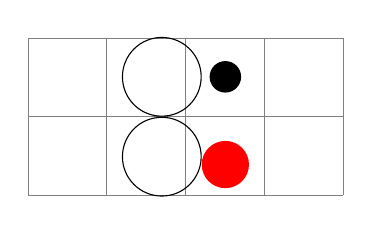
\begin{tikzpicture}
  \draw[help lines] (0,0) grid (4,2);
  \node [matrix] at (2,1)
  {
    \draw (0,0)   circle (5mm); & \fill      (0,0) circle (2mm); \\
    \draw (0,0.1) circle (5mm); & \fill[red] (0,0) circle (3mm); \\
  };
\end{tikzpicture}
\end{codeexample}
\end{itemize}


%%% Local Variables: 
%%% mode: latex
%%% TeX-master: "pgfmanual"
%%% End: 
